\documentclass[11pt, spanish, a4paper, twoside]{article}
% Versión 1.er cuat 2021 Víctor Bettachini < bettachini@df.uba.ar >

% Versión 1.er cuat 2021 Víctor Bettachini < bettachini@df.uba.ar >

\usepackage[T1]{fontenc}
\usepackage[utf8]{inputenc}

\usepackage[spanish, es-tabla]{babel}
\def\spanishoptions{argentina} % Was macht dass?
% \usepackage{babelbib}
% \selectbiblanguage{spanish}
% \addto\shorthandsspanish{\spanishdeactivate{~<>}}

\usepackage{graphicx}
\graphicspath{{./figuras/}{../LaTeX/}}
% \usepackage{float}

\usepackage[arrowdel]{physics}
\newcommand{\pvec}[1]{\vec{#1}\mkern2mu\vphantom{#1}}
% \usepackage{units}
\usepackage[separate-uncertainty=true, multi-part-units=single, locale=FR]{siunitx}
\usepackage{isotope} % $\isotope[A][Z]{X}\to\isotope[A-4][Z-2]{Y}+\isotope[4][2]{\alpha}

\usepackage{tasks}
\usepackage[inline]{enumitem}
% \usepackage{enumerate}

\usepackage{hyperref}

% \usepackage{amsmath}
% \usepackage{amstext}
\usepackage{amssymb}

\usepackage{tikz}
\usepackage{tikz-dimline}
\usetikzlibrary{calc}
% \usetikzlibrary{math}
\usetikzlibrary{arrows.meta}
\usetikzlibrary{snakes}
\usetikzlibrary{decorations}
\usetikzlibrary{decorations.pathmorphing}
\usetikzlibrary{patterns}

% \usepackage[hmargin=1cm, vmargin=1cm, includeheadfoot]{geometry}
\usepackage[hmargin=1cm,vmargin=3cm, top= 0.75cm,nohead]{geometry}
% \voffset-3.5cm
% \hoffset-3cm
% \setlength{\textwidth}{17.5cm}
% \setlength{\textheight}{27cm}

\usepackage{lastpage}
\usepackage{fancyhdr}
\pagestyle{fancyplain}
\fancyhf{}
% \fancyhead{}
\setlength\headheight{28.7pt} 
\fancyhead[LE, LO]{\textbf{Física 2} (Físicos) }
% \lhead{\textbf{Física 2} (Físicos) }
\fancyhead[RE, RO]{\href{https://df.uba.ar/es/}{$\vcenter{\hbox{
\includegraphics[height=1cm]{sin_texto.pdf}}}$}}
% \rhead{$\vcenter{\hbox{
\includegraphics[height=1cm]{sin_texto.jpg}}}$}
% \rhead{
\includegraphics[height=1cm]{sin_texto.jpg}}
% \rhead{\textcopyright {\tt DF, FCEyN, UBA}}
\fancyfoot{\href{https://creativecommons.org/licenses/by-sa/4.0/deed.es/}{$\vcenter{\hbox{
\includegraphics[height=0.4cm]{cc-by-sa.pdf}}}$} \href{https://df.uba.ar/es/}{DF, FCEyN, UBA}}
% \fancyfoot{$\vcenter{\hbox{
\includegraphics[height=0.4cm]{cc-by-sa.pdf}}}$ DF, FCEyN, UBA}
% \fancyfoot{{\tiny \textcopyright DF, FCEyN, UBA}}
\fancyfoot[C]{ {\tiny Actualizado al \today} }
\fancyfoot[RO, LE]{Pág. \thepage/\pageref{LastPage}}
\renewcommand{\headrulewidth}{0pt}
\renewcommand{\footrulewidth}{0pt}


\begin{document}
\begin{center}
	% \textbf{Física 2} (Físicos) \hfill \textcopyright {\tt DF, FCEyN, UBA}\\
	\textsc{\LARGE Propagación de la luz}
\end{center}

Los ejercicios con (*) entrañan una dificultad adicional. Son para investigar después de resolver los demás.


\begin{enumerate}

\section*{Prisma}

\item
\begin{enumerate}
	\item Un haz de luz monocromático al atravesar un prisma cambia su dirección en un ángulo de desviación \(\delta \alpha\).
	Haga un gráfico cualitativo que le permita ver el efecto sobre \(\delta \alpha\) del ángulo con que incidió en las cara que numeraremos 1.
	Para esto dibuje dos casos de ángulos respecto a la normal de esa cara \(\theta_{i1}\) bien distintos.
	\item Calcule analíticamente el ángulo de desviación mínima \(\delta \alpha_\text{mín}\) para un prisma en función de los datos constructivos.
\end{enumerate}


\item
\begin{enumerate}
	\item En un vidrio óptico común se propaga un haz de luz blanca, ¿qué componente viaja más rápido: la roja o la violeta?
	\item ¿Para cuál de ambos colores será mayor la desviación en un prisma \(\delta \alpha_n\) ?
	¿Qué puede decir del ángulo de desviación mínima \(\delta \alpha_\text{mín}\)?
\end{enumerate}



\item Dado un prisma de \emph{vidrio Crown} de ángulo $\alpha = \ang{4;;}$ calcular, para las \emph{líneas de absorción de Fraunhofer} F, D\textsubscript{1} y C, las desviaciones de rayos que inciden casi perpendicularmente.
Los respectivos índices son: $n_F = 1.513$; $n_D = 1.508$ y $n_C =1.504$.


\section*{Reflexión total interna}

\item Verifique o demuestre que:\\
\begin{minipage}[t][4.5cm]{0.65\textwidth}
\begin{enumerate}
	\item Un rayo que incide sobre una lámina de caras paralelas, inmersa en un medio único, no se desvía al atravesarla.
	Calcule el desplazamiento lateral \(\Delta\) de dicho rayo, en términos de su espesor \(d\) y de su índice de refracción \(n\)
	\item El rayo que se refleja en la primera cara y el que emerge luego de reflejarse en la segunda son paralelos.
\end{enumerate}
Si el medio exterior es único, ¿existe un ángulo de incidencia que produzca reflexión total en la cara inferior?
\end{minipage}
\begin{minipage}[c][0cm][t]{0.33\textwidth}
	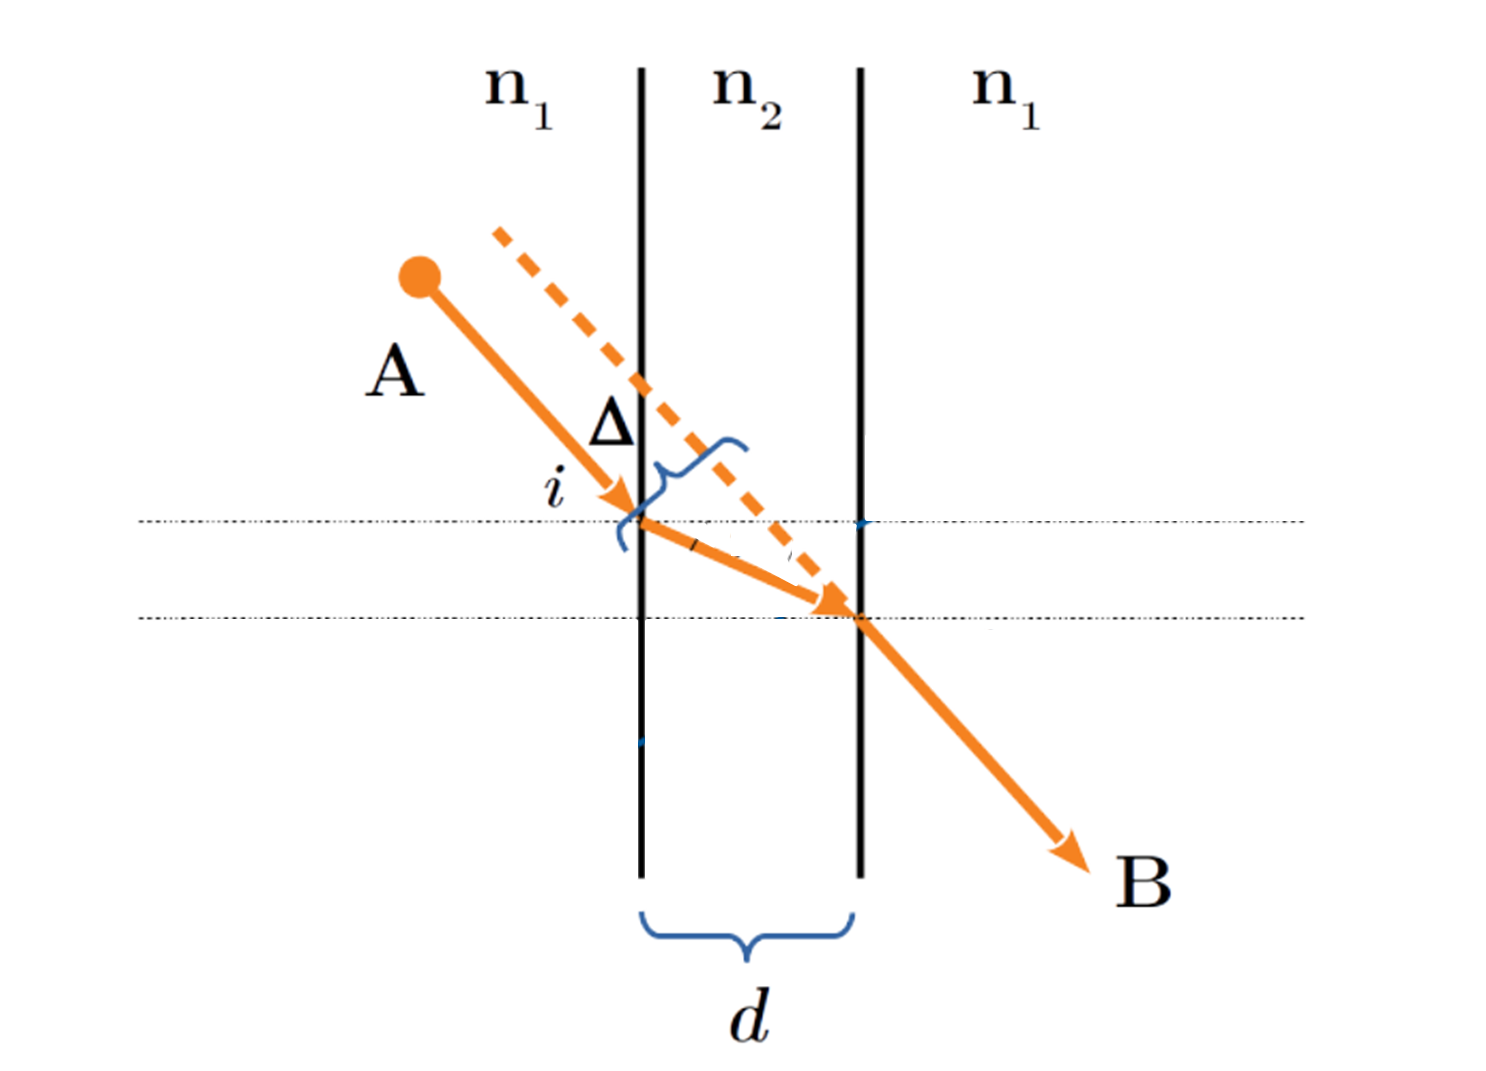
\includegraphics[width=\textwidth]{a-000}
\end{minipage}




\item (*)
\begin{minipage}[t][3.5cm]{0.75\textwidth}
Un rayo incide con ángulo $\phi$ sobre la superficie horizontal de un cubo de material transparente, de índice $n$, inmerso en aire.
\begin{enumerate}
	\item ¿Para qué valores de $\phi$ hay reflexión total en la cara vertical?
	\item Si $\phi=60^{\circ}$, ¿cuál es el máximo $n$ para que no haya reflexión total en la cara vertical?
	¿Se puede reflejar totalmente en la cara superior?
\end{enumerate}
\end{minipage}
\begin{minipage}[c][1.5cm][t]{0.15\textwidth}
	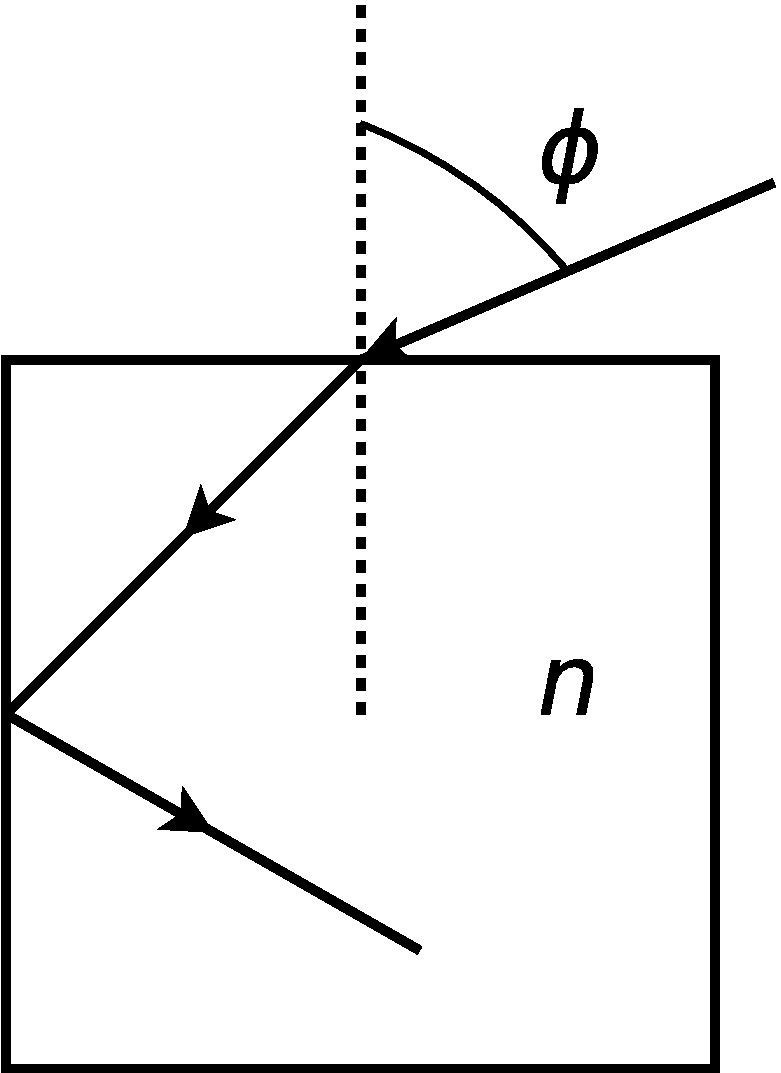
\includegraphics[width=\textwidth]{ej3-5}
\end{minipage}



\item
La fibra óptica es en esencia una hebra muy fina de un material de alto índice de refracción, e.g. cristal de silicio o plástico transparente.
Un revestimiento (\emph{cladding}) de menor índice logra, por reflexión total, que la luz que ingresa por un extremo al núcleo (\emph{core}) solo pueda salir por el otro.
\begin{figure}[ht]
	\centering{}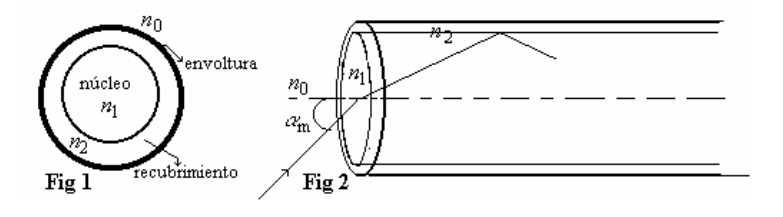
\includegraphics[width=0.75\textwidth]{fibra}
\end{figure}
\begin{enumerate}
	\item Verifique que sufren reflexión total los rayos dentro del ángulo \(\alpha_A\) del cono de aceptación. 
	\[
		\sen{(\alpha_A)} = \frac{n_1}{n_o} \sqrt{1- \left( \frac{n_2}{n_1} \right)^2 }
	\]
	siendo \(n_0\), \(n_1\) y \(n_2\) índices de refracción del medio exterior, núcleo y recubrimiento.
	\item Como el cono de aceptación depende del índice que rodea a la fibra en el extremo de entrada, suele emplearse la magnitud denominada apertura numérica que se define como
	\[
		\text{AN} = n \sen{(\alpha_A)}
	\]
	Calcule la apertura numérica correspondiente a una fibra cuyo núcleo tiene un índice de refracción de \num{1.66} y el correspondiente a su recubrimiento es \num{1.4}.
	Para estos valores, ¿cuál es el ángulo de aceptación si la luz proviene del aire? ¿Y si proviene del agua?
	\item ¿Qué rango de valores debería tener el índice de refracción del recubrimiento de un núcleo cuyo índice es \num{1.66} para que todo rayo que incida desde el aire quede atrapado dentro de la fibra?
\end{enumerate}



\item Los índices de refracción de cierta clase de vidrio para el rojo y el violeta valen: $1.51$ y $1.53$; respectivamente.
Halle los ángulos límites de reflexión total para rayos que incidan en la superficie de separación vidrio-aire.
¿Qué ocurre si un rayo de luz blanca incide formando un ángulo de 41$^{\circ}$ sobre dicha superficie?




\end{enumerate}

\end{document}
